% Options for packages loaded elsewhere
\PassOptionsToPackage{unicode}{hyperref}
\PassOptionsToPackage{hyphens}{url}
\PassOptionsToPackage{dvipsnames,svgnames,x11names}{xcolor}
%
\documentclass[
  a4paper]{article}

\usepackage{amsmath,amssymb}
\usepackage{iftex}
\ifPDFTeX
  \usepackage[T1]{fontenc}
  \usepackage[utf8]{inputenc}
  \usepackage{textcomp} % provide euro and other symbols
\else % if luatex or xetex
  \usepackage{unicode-math}
  \defaultfontfeatures{Scale=MatchLowercase}
  \defaultfontfeatures[\rmfamily]{Ligatures=TeX,Scale=1}
\fi
\usepackage{lmodern}
\ifPDFTeX\else  
    % xetex/luatex font selection
\fi
% Use upquote if available, for straight quotes in verbatim environments
\IfFileExists{upquote.sty}{\usepackage{upquote}}{}
\IfFileExists{microtype.sty}{% use microtype if available
  \usepackage[]{microtype}
  \UseMicrotypeSet[protrusion]{basicmath} % disable protrusion for tt fonts
}{}
\makeatletter
\@ifundefined{KOMAClassName}{% if non-KOMA class
  \IfFileExists{parskip.sty}{%
    \usepackage{parskip}
  }{% else
    \setlength{\parindent}{0pt}
    \setlength{\parskip}{6pt plus 2pt minus 1pt}}
}{% if KOMA class
  \KOMAoptions{parskip=half}}
\makeatother
\usepackage{xcolor}
\usepackage[margin=1in]{geometry}
\setlength{\emergencystretch}{3em} % prevent overfull lines
\setcounter{secnumdepth}{5}
% Make \paragraph and \subparagraph free-standing
\ifx\paragraph\undefined\else
  \let\oldparagraph\paragraph
  \renewcommand{\paragraph}[1]{\oldparagraph{#1}\mbox{}}
\fi
\ifx\subparagraph\undefined\else
  \let\oldsubparagraph\subparagraph
  \renewcommand{\subparagraph}[1]{\oldsubparagraph{#1}\mbox{}}
\fi


\providecommand{\tightlist}{%
  \setlength{\itemsep}{0pt}\setlength{\parskip}{0pt}}\usepackage{longtable,booktabs,array}
\usepackage{calc} % for calculating minipage widths
% Correct order of tables after \paragraph or \subparagraph
\usepackage{etoolbox}
\makeatletter
\patchcmd\longtable{\par}{\if@noskipsec\mbox{}\fi\par}{}{}
\makeatother
% Allow footnotes in longtable head/foot
\IfFileExists{footnotehyper.sty}{\usepackage{footnotehyper}}{\usepackage{footnote}}
\makesavenoteenv{longtable}
\usepackage{graphicx}
\makeatletter
\def\maxwidth{\ifdim\Gin@nat@width>\linewidth\linewidth\else\Gin@nat@width\fi}
\def\maxheight{\ifdim\Gin@nat@height>\textheight\textheight\else\Gin@nat@height\fi}
\makeatother
% Scale images if necessary, so that they will not overflow the page
% margins by default, and it is still possible to overwrite the defaults
% using explicit options in \includegraphics[width, height, ...]{}
\setkeys{Gin}{width=\maxwidth,height=\maxheight,keepaspectratio}
% Set default figure placement to htbp
\makeatletter
\def\fps@figure{htbp}
\makeatother

\makeatletter
\makeatother
\makeatletter
\makeatother
\makeatletter
\@ifpackageloaded{caption}{}{\usepackage{caption}}
\AtBeginDocument{%
\ifdefined\contentsname
  \renewcommand*\contentsname{Table of contents}
\else
  \newcommand\contentsname{Table of contents}
\fi
\ifdefined\listfigurename
  \renewcommand*\listfigurename{List of Figures}
\else
  \newcommand\listfigurename{List of Figures}
\fi
\ifdefined\listtablename
  \renewcommand*\listtablename{List of Tables}
\else
  \newcommand\listtablename{List of Tables}
\fi
\ifdefined\figurename
  \renewcommand*\figurename{Figure}
\else
  \newcommand\figurename{Figure}
\fi
\ifdefined\tablename
  \renewcommand*\tablename{Table}
\else
  \newcommand\tablename{Table}
\fi
}
\@ifpackageloaded{float}{}{\usepackage{float}}
\floatstyle{ruled}
\@ifundefined{c@chapter}{\newfloat{codelisting}{h}{lop}}{\newfloat{codelisting}{h}{lop}[chapter]}
\floatname{codelisting}{Listing}
\newcommand*\listoflistings{\listof{codelisting}{List of Listings}}
\makeatother
\makeatletter
\@ifpackageloaded{caption}{}{\usepackage{caption}}
\@ifpackageloaded{subcaption}{}{\usepackage{subcaption}}
\makeatother
\makeatletter
\@ifpackageloaded{tcolorbox}{}{\usepackage[skins,breakable]{tcolorbox}}
\makeatother
\makeatletter
\@ifundefined{shadecolor}{\definecolor{shadecolor}{rgb}{.97, .97, .97}}
\makeatother
\makeatletter
\makeatother
\makeatletter
\makeatother
\ifLuaTeX
  \usepackage{selnolig}  % disable illegal ligatures
\fi
\usepackage[]{biblatex}
\addbibresource{bibliography.bib}
\nocite{*}
\IfFileExists{bookmark.sty}{\usepackage{bookmark}}{\usepackage{hyperref}}
\IfFileExists{xurl.sty}{\usepackage{xurl}}{} % add URL line breaks if available
\urlstyle{same} % disable monospaced font for URLs
\hypersetup{
  pdftitle={Bitcoin sentiment analysis},
  pdfauthor={Ambroise Thibault, Faune Blanchard, Maxime Lorenzo},
  colorlinks=true,
  linkcolor={blue},
  filecolor={Maroon},
  citecolor={Blue},
  urlcolor={Blue},
  pdfcreator={LaTeX via pandoc}}

\title{Bitcoin sentiment analysis}
\author{Ambroise Thibault, Faune Blanchard, Maxime Lorenzo}
\date{}

\begin{document}
\maketitle
\ifdefined\Shaded\renewenvironment{Shaded}{\begin{tcolorbox}[boxrule=0pt, sharp corners, frame hidden, enhanced, borderline west={3pt}{0pt}{shadecolor}, breakable, interior hidden]}{\end{tcolorbox}}\fi

\renewcommand*\contentsname{Table of contents}
{
\hypersetup{linkcolor=}
\setcounter{tocdepth}{4}
\tableofcontents
}
\hypertarget{introduction}{%
\section{Introduction}\label{introduction}}

This project asks a simple question: can the mood of the market help us
make better decisions when trading cryptocurrencies? We adapted a
research paper called Ghost in the Machine \textcite{leland_bybee_2025},
which showed that in traditional markets, sentiment often builds up
before a crash. That made us wonder if we could take similar ideas and
apply them to crypto, which is even more emotional and unpredictable.
The goal was to see if tracking sentiment could help us understand how
prices are going to move. Often, crypto naysayers say that
cryptocurrency prices rely on nothing but speculation. Therefore, trying
to understand the market's ``irrational'' response to news can help shed
light on this debate. Even though it doesn't resolve the core question
of the intrinsic value of bitcoin, it can show if investors in
cryptocurrency are more or less emotional than investors in ``classic''
assets.

We started by collecting sentiment data from places like news headlines.
The idea was to measure whether the overall tone on a given day was
positive, negative, or somewhere in between. For this, we used the
methodology presented in the paper, which we adapted to work with
Mistral AI (the Large Language Model (LLM) developed by french startup
Mistral), which is cheaper and easier to scale than GPT 3.5 (the LLM
used in the paper). Feeding the headlines to the LLM helped us develop a
time series of a sentiment ``score'' going from -1 to 1, which we can
then compare to bictoin returns using a logistic regression. Then, we
improve the results from this regression by using the ex-ante residuals
(EAR, more information later) of the scores instead. We found that the
EAR slightly improves the results from the logistic regression, although
both methods beat randomness.

After that, we apply an impulse reaction function (IRF, to be defined
later) to create a trading signal on Bitcoin, and compare the results
with a simple long bitcoin portfolio. We find that this trading strategy
gives much better results in theory. We reiterate once again that the
combination or the EAR and the IRF comes entirely from the paper we
decided to adapt, although it doesn't use the logistic regressions like
we did.

\hypertarget{background}{%
\section{Background}\label{background}}

\hypertarget{what-is-sentiment-why-is-it-important-in-cryptocurrencies-compared-to-traditional-assets}{%
\subsection{What is sentiment ? Why is it important in cryptocurrencies
compared to traditional assets
?}\label{what-is-sentiment-why-is-it-important-in-cryptocurrencies-compared-to-traditional-assets}}

In finance, market sentiment (or investor sentiment) refers to the
general attitude or mood of investors towards a market or asset. It
reflects crowd psychology and often manifests itself in trading
behavior: optimism (bullish sentiment) can trigger frenzied buying,
while fear (bearish sentiment) leads to massive selling. It is essential
to note that sentiment is distinct from fundamentals: it refers to
emotions and perceptions rather than intrinsic value. In equity markets,
sentiment can drive prices well above or below what fundamental
valuation suggests.

Bitcoin and other cryptocurrencies do not have any financial reports,
cash flows or earnings needed for traditional fundamental analysis,
unlike equities or bonds. Their value is largely speculative, so the
emotional state of the market plays a disproportionate role. Thus, news,
tweets and online discussions can move crypto prices quickly and
strongly. Elon Musk's tweets, for example, have caused Bitcoin or
Dogecoin to soar, illustrating how media hype or fear on social media
translates into market volatility. The characteristics of the crypto
market amplify these effects: it trades 24/7 and it's heavily dominated
by retail investors on a global scale. This investor base, generally
less experienced and more versatile than traditional investors, allows
positive or negative opinions to spread like contagion in these still
immature markets. The result is rapid herding behavior, with investors
buying collectively in euphoria or selling in panic, thereby
accentuating volatility.

Several key distinctions make sentiment dynamics unique in crypto
compared to equities or other traditional assets. Firstly, traditional
equities rely on fundamentals (earnings, dividends) that anchor
long-term value, whereas Bitcoin's value is essentially shaped by a
narrative. Crypto prices can therefore fluctuate much more wildly on
sentiment alone. Equity markets certainly go through speculative phases,
but extreme sentiment is partly tempered by fundamental outlook. In
crypto, a meme or a rumor can spark a buying frenzy without concrete
support. This is why indicators such as the Crypto Fear \& Greed Index
(inspired by CNN's index for stocks) are closely scrutinized: they
aggregate volatility, volumes and social network sentiment to offer a
unique barometer of market mood.

Secondly, unlike stock exchanges, crypto markets operate without
interruption on a global scale. There's no ``weekend break'' to digest
news, so sentiment can build continuously. A viral tweet at 3 a.m. can
trigger immediate reactions all over the world. The decentralized nature
of the system means that information and sentiment spread via social
networks (Twitter/X, Reddit, Telegram) rather than through official
channels. This democratization of the information flow makes investor
sentiment both highly reactive and widely distributed, unlike
conventional markets where institutional investors can moderate sudden
movements.

Finally, crypto assets are often associated with online subcultures
(Bitcoin on Twitter, Dogecoin on Reddit, etc.). The tone of these
communities directly influences market behavior. Individual traders
frequently rally to a collective sentiment, a less common phenomenon for
``blue chip'' stocks. Jargon and memes embody sentiment-driven
investment philosophies specific to crypto. These emotional drivers are
less present in traditional assets (excluding recent episodes of ``meme
stocks'').

In short, sentiment is a key driver for Bitcoin, as its valuation relies
on investor narrative and momentum. While sentiment also affects stocks
and bonds, these markets have established mechanisms and fundamentals
that cushion the impact. Crypto-currencies, on the other hand, move
largely on sentiment-driven momentum, hence the importance of analyzing
social media sentiment to understand and predict Bitcoin's price
movements.

\hypertarget{sentiment-analysis-and-llms}{%
\subsection{Sentiment analysis and
LLMs}\label{sentiment-analysis-and-llms}}

\hypertarget{what-are-llms-how-are-they-useful-for-sentiment-analysis}{%
\subsubsection{What are LLMs ? How are they useful for sentiment
analysis
?}\label{what-are-llms-how-are-they-useful-for-sentiment-analysis}}

Large Language Models (LLMs) are advanced neural networks with an
extremely high number of parameters (often billions) trained on huge
text corpora. Modern LLMs learn the statistical patterns of language,
enabling them to generate and understand text with remarkable ease.
Notable examples include OpenAI's GPT series, Google's PaLM and Meta's
LLaMA. These models show impressive performance on a wide range of
natural language processing tasks (from translation to question
answering) without task-specific training, relying on the knowledge
encoded during pre-training. In concrete terms, an LLM can be given a
prompt, and will then produce a human-quality text or classify the
sentiment of a passage thanks to its general understanding of language.

LLMs' ability to capture context makes them powerful tools for sentiment
analysis. Previous approaches often struggled with nuances such as
sarcasm, idioms or domain-specific jargon. Trained on a variety of
internet texts (forums, news, social media), LLMs are better equipped to
interpret these subtleties. In general, LLM-based sentiment analysis
does not rely on manual lists of positive/negative words but rather
relies on a learned representation of language. LLMs can thus detect
feelings present in complex sentences, frequent in crypto discussions.
Their extensive training also gives them a vast store of contextual
knowledge. These capabilities make LLMs especially suited to analyzing
social media posts about Bitcoin, which often include informal language,
emojis, and evolving jargon.

LLMs also offer practical advantages: being generalists, the same model
can be applied to various sentiment tasks with a minimum of adaptation.
For example, an LLM can be asked: ``classify the sentiment of this
tweet'' and get a relevant answer without training a new model for weeks
on an annotated dataset. In finance, specialized LLMs have even been
created to increase accuracy: FinBERT, a BERT-like model refined
(fine-tuned) on financial texts, is one of the best known.

In short, LLMs have become indispensable for sentiment analysis: they
combine width (pre-training on huge data sets covering multiple
sentiment expressions) and depth (neural architectures capable of
capturing subtle linguistic patterns). They excel at understanding
context, sarcasm and fine emotions, omnipresent in the sentiment
conveyed on social networks about cryptocurrencies. Moreover, they can
process huge volumes of data - analyzing thousands of tweets or forum
comments to tease out the general trend in sentiment - making them
particularly useful for tracking the mood around Bitcoin on Twitter,
Reddit, etc., with a level of nuance that previous approaches couldn't
achieve.

\hypertarget{limits-of-llms}{%
\subsubsection{Limits of LLMs}\label{limits-of-llms}}

While LLMs represent state-of-the-art technology, it's important to
critically assess their limitations, especially in a sensitive
application like financial sentiment analysis:

Firstly, unlike lexicons or logistic regression models, which offer a
degree of interpretability (we can see which words are counted as
positive or negative), LLMs are black boxes. When a model labels a tweet
as positive or negative, it's difficult to extract a
human-understandable rationale. This can be problematic in an academic
or professional setting, where the analyst needs to explain why a
sentiment is reported in a certain way.

Another disadvantage is that LLM responses can vary according to the
wording of the task. Slight changes in wording can produce different
results, undermining the consistency of an automated analysis. Reliable
sentiment analysis in production therefore requires carefully designed
prompts or fine-tuning, failing which the model can sometimes deviate
(giving a long explanation and then, the next time, a single word, or
misinterpreting a request). Imposing uniform criteria for sentiment
(e.g.~always returning ``Positive/Neutral/Negative'') requires
particular care in prompt design or model tuning.

LLMs are also resource-hungry. Running GPT-4 on thousands of messages
can be slow and costly compared to a lighter algorithm. In real-time
trading scenarios, the latency of a large model can be too high:
microsecond decisions can't wait for a model with several billion
parameters to process the text. Access to the latest LLMs also involves
API costs or infrastructure that may be out of reach. At large scale
(continuous analysis of every tweet on Bitcoin), the use of an LLM can
therefore be expensive.

In conclusion, LLMs are powerful but not infallible tools. They need to
be handled with care: watch out for biases, test for contextual pitfalls
(such as sarcasm) and anticipate their resource requirements. Knowing
these limitations (e.g.~misinterpretation, bias, opacity, inconsistency,
cost and knowledge gaps, etc) enables us to better exploit the strengths
of LLMs while mitigating their weaknesses for analyzing social network
sentiment around Bitcoin. Although we still use them in this project, we
need to specify that this is a flawed tool and that our model has clear
weaknesses.

\hypertarget{generating-sentiment-score}{%
\section{Generating sentiment score}\label{generating-sentiment-score}}

\hypertarget{presentation-of-the-database}{%
\subsection{Presentation of the
database}\label{presentation-of-the-database}}

We collected a dataset from GitHub entitled
\href{https://github.com/soheilrahsaz/cryptoNewsDataset}{Crypto News
Dataset}. It aggregates daily headlines from a variety of crypto news
websites. Each headline is labeled with the cryptocurrencies to which it
refers. They are also timestamped down to the second the news was posted
on the site. We also have the number of likes, dislikes, comments and
others, although these are often 0, as well as the link to the article.
In this project, we will only be using the raw headlines in order to
generate the scores that we need.

Here is a quick view of the pre processed dataset with our function
``import\_data'' in the ``prompts'' module. This function reads the csv
files from the GitHub repository linked above, then it removes unwanted
columns and formats the date so that we only have the day at which it
was posted. We can see that there can be multiple headlines in one day,
or no headlines. This will cause issues that we will explain later on in
the project.

The function also writes the prompts that we will later feed to the
Large Language Model in order to properly generate the scores, which we
will explain in the following section.

\hypertarget{generating-prompts}{%
\subsection{Generating prompts}\label{generating-prompts}}

For each headline, we generate a prompt which asks the AI its beliefs
about the evolution of Bitcoin returns based on this headline. The
prompt we decided to use is the exact prompt presented in
\textcite{leland_bybee_2025} . The exact prompt reads :

\begin{verbatim}
Here is a piece of news:
"%s"
Do you think this news will increase or decrease BTC?
Write your answer as: 
{increase/decrease/uncertain}:
{confidence (0-1)}:
{magnitude of increase/decrease (0-1)}:
{explanation (less than 25 words)}
\end{verbatim}

Where ``\%s'' is replaced by the headline. After editing this prompt, we
notice that removing part of this prompt changes the results drastically
(from ``increase'' to ``decrease'' for the same headline). Therefore, we
decided to keep the prompt from the paper as is, even though we will
only use the results for ``increase'' or ``decrease'' for this project.
This prompt has been adapted from traditional retail investor surveys or
surveys of CFOs that are used to produce a sentiment indicator. However,
these are costly and slow. As presented in the paper, using AI models to
replace human answers mimics the same results on a much bigger and
faster scale.

More information about the construction on this prompt can be found in
\textcite{leland_bybee_2025} .

Here, we use the Mistral LLM to generate prompt answers. The Mistral AI
API is a service that gives us access to powerful language models,
similar to ChatGPT or Claude. These models can read and interpret text,
making them useful for tasks like summarizing news or detecting the tone
of an article. In our project, we use the Mistral API to process
financial headlines or crypto-related news and ask the model the prompt
presented earlier. The model then gives us a structured answer,
including its level of confidence and a short explanation.

Running sentiment scoring at a large scale using the Mistral API isn't
just about sending a bunch of text to a model. It quickly becomes a
technical challenge. If you're processing thousands (or even millions)
of headlines, you need to manage API requests carefully. Language models
are slow compared to normal scripts, and APIs often have strict rate
limits. If you send too many requests too fast, you'll get throttled or
even temporarily blocked. That means you need to build in delays, handle
retries, and keep track of how many requests you're sending per second
or minute.

To make this efficient, the code has to handle asynchronous execution
and concurrency. Instead of sending requests one by one (which would
make the code very inefficient and take a long time to generate
answers), we wanted to send many in parallel---without breaking the API
rules. That means using tools like Python's asyncio, aiohttp, or httpx,
and writing logic that can pause, retry failed calls, and wait when
needed. WWe however also needed to track which headlines have already
been scored to handle failures cleanly. Scaling this up without crashing
the system or getting banned by the API meant taking additional security
measures in the code.

For a detailed overview of the steps we decided to take, please refer to
the notebook ``sandbox\_ambroise.ipynb'' on our github repository
(faunebl/crypto-sentiment).

\hypertarget{scores-methodology}{%
\subsection{Scores methodology}\label{scores-methodology}}

After getting the scores from the LLM, we are left with categorical
values for each news, while there are multiple news per day. Therefore,
we decide to assign 1 if the LLM says the news will increase BTC, -1 if
it says it will decrease, and if it is uncertain we will ignore the
headline entirely (so as to not create noise). Then, we aggregate every
headline for one day, so that we get a clean series with one sentiment
score per day. To aggregate, we use the formula presented in the paper:

\[
F^\text{gpt}_t *(X^k_{t+h}) = \frac{\sum_{i \in \mathcal{A}_t} \mathbb{I}(\text{Increase}^k_i) - \mathbb{I}(\text{Decrease}^k_i)}{\sum_{i \in \mathcal{A}_t} \mathbb{I}(\text{Increase}^k_i) + \sum_{i \in \mathcal{A}_t} \mathbb{I}(\text{Decrease}^k_i)}
\]

The EAR, or Ex-Ante Residual, is meant to capture the part of sentiment
that can't be predicted based on past patterns. We do this by using a
simple model (like anautoregressive model i.e.~AR(1)): a linear
regression where the explanatory variable is simply the lagged target)
to see what today's sentiment should be, based on yesterday's.
Whatever's left over (i.e.~the part the AR(1) model didn't expect) is
the EAR. It's the surprise in the mood of the market. Here is how it is
constructed mathematically:

\begin{enumerate}
\def\labelenumi{\arabic{enumi}.}
\item
  We first compute an autoregressive model of sentiment (based on the
  score presented earlier):
  \(\text{Sentiment}_t = \alpha + \beta \cdot \text{Sentiment}_{t-1} + \varepsilon_t\)
\item
  Then, we compute the residuals for that model:
  \(\text{EAR}_t = \text{Sentiment}_t - (\alpha + \beta \cdot \text{Sentiment}_{t-1})\)
\end{enumerate}

This surprise is important because it often reflects emotional or
irrational shifts. In crypto especially, people can get overly excited
or scared in ways that don't line up with the data. By focusing on these
unexpected jumps in sentiment, we're trying to isolate the moments when
crowd psychology might be taking over---when prices could be getting
ahead of reality.

\hypertarget{comparison-with-btc-returns}{%
\section{Comparison with BTC
returns}\label{comparison-with-btc-returns}}

\hypertarget{introduction-1}{%
\subsection{Introduction}\label{introduction-1}}

To extract the returns, we use the yahoo finance
\textcite{yahoo_finance} API. The details for this can be found in the
get\_btc\_returns function of the utils.py module in our github
repository.

We use this introduction to give a little bit of background about the
logistic regression. It functions as a normal linear regression, except
that it applied a sigmoid function to the results in order to predict a
binary outcome. Here the binary outcome is :

\begin{enumerate}
\def\labelenumi{\arabic{enumi}.}
\item
  \(\text{Return}_t > 0\)
\item
  \(\text{Return}_t < 0\)
\end{enumerate}

Which works because it is almost impossible that the logarithmic returns
are exactly zero. In this context, we will only have one predictor
variable (i.e.~X is one-dimensional), which will alternatively be the
raw scores and then the EAR. Therefore, the formula for the logistic
regression is :

\[
P(Y = 1 \mid X) = \frac{1}{1 + e^{-(\beta_0 + \beta_1 X)}}
\]

Which means that the probability that Y is 1 given the current value of
X is the sigmoid (i.e., a function that yields a discrete number from a
continuous value) of the result of simple linear regression. Here
\(\beta_0\) and \(\beta_1\) are computed with the usual linear
regression formula (that we don't recall here for readability purposes).

We interpret the results of a logistic regression thanks to a confusion
matrix, accuracy, precision and recall.

A \textbf{\emph{confusion matrix}} helps you understand how well your
model is doing at making predictions by showing four outcomes: true
positives (correctly predicted positives), true negatives (correctly
predicted negatives), false positives (incorrectly predicted positives),
and false negatives (positives that weren't detexted).
\textbf{\emph{Accuracy}} tells you the overall percentage of correct
predictions. \textbf{\emph{Precision}} tells you, out of all the times
the model predicted ``yes,'' how many were actually correct (useful when
false alarms are costly). \textbf{\emph{Recall}} tells you, out of all
the actual ``yes'' cases, how many the model correctly caught (important
when missing positives is risky).

\hypertarget{comparing-with-scores}{%
\subsection{Comparing with scores}\label{comparing-with-scores}}

\hypertarget{results}{%
\subsubsection{Results}\label{results}}

We first show what the scores look like in time.

\begin{figure}

{\centering 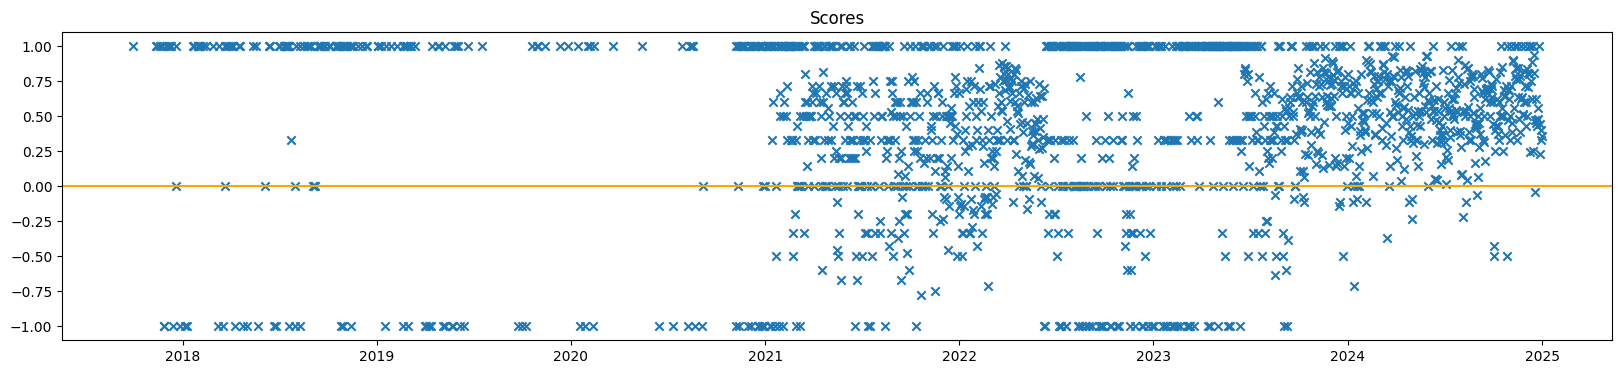
\includegraphics{graphs/scores_vs_time.png}

}

\caption{Scores vs time}

\end{figure}

We can see that, once we have a bit more data about BTC headlines, the
scores start being different from just 1 or -1. Indeed, if we have only
one or two headlines, it is sufficient that only one is positive to get
a score of 1. This is why the model might be biased during training,
although we have no way or overcoming this with the current dataset.

We also look at the distribution of the scores:

\begin{figure}

{\centering 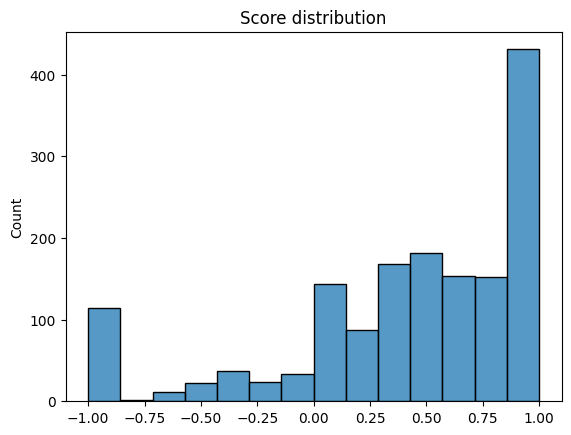
\includegraphics[width=2.60417in,height=\textheight]{graphs/scores_distrib.png}

}

\end{figure}

We can see a strong skew towards 1. This is particularly problematic
when we compare the distribution of the returns of BTC:\\

\begin{figure}

{\centering 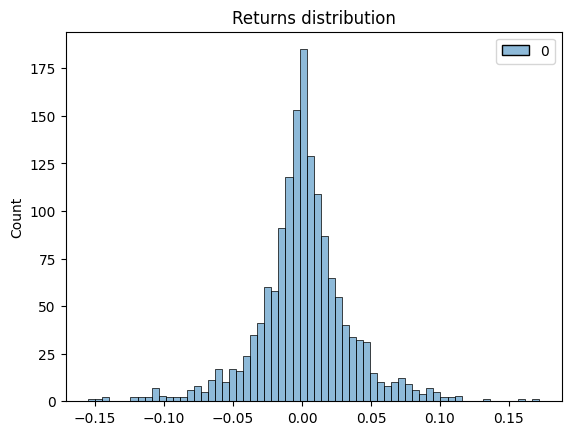
\includegraphics[width=2.60417in,height=\textheight]{graphs/Returns distribution.png}

}

\caption{BTC returns distribution}

\end{figure}

We have to look at the tails of this distribution because we will
binarize this and regress on if returns are positive or negative. We can
plot the tails:

\begin{figure}

{\centering 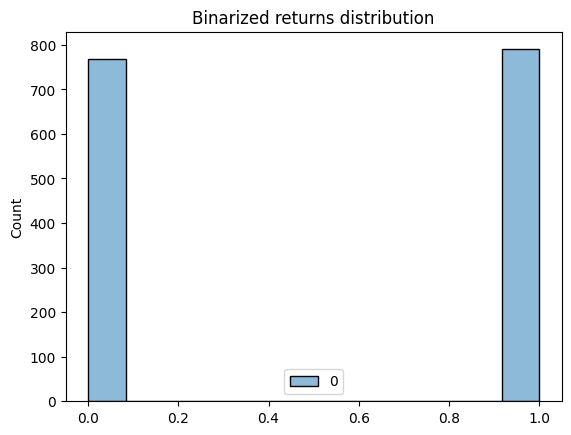
\includegraphics[width=2.60417in,height=\textheight]{graphs/binary_distrib.png}

}

\caption{Binary distribution}

\end{figure}

Here, we can see that both classes are equal. This is partly why we
decided to use a logistic regression instead of a simple binarizer model
(which would've been, if scores \textgreater{} 0 then we say that
returns \textgreater{} 0). We would have introduced a bias because of
this difference in class distribution.

We then present the scores for the results:

\begin{table}[h]
\centering
\begin{tabular}{|l|c|c|c|c|}
\hline
\textbf{Dataset} & \textbf{Accuracy} & \textbf{Precision} & \textbf{Recall} & \textbf{F1 Score} \\
\hline
In Sample      & 0.5269 & 0.5270 & 0.5269 & 0.5255 \\
Out of Sample  & 0.5318 & 0.5318 & 0.5318 & 0.4984 \\
\hline
\end{tabular}
\caption{Model performance metrics in and out of sample}

\end{table}

And the confusion matrix :

\begin{figure}

{\centering 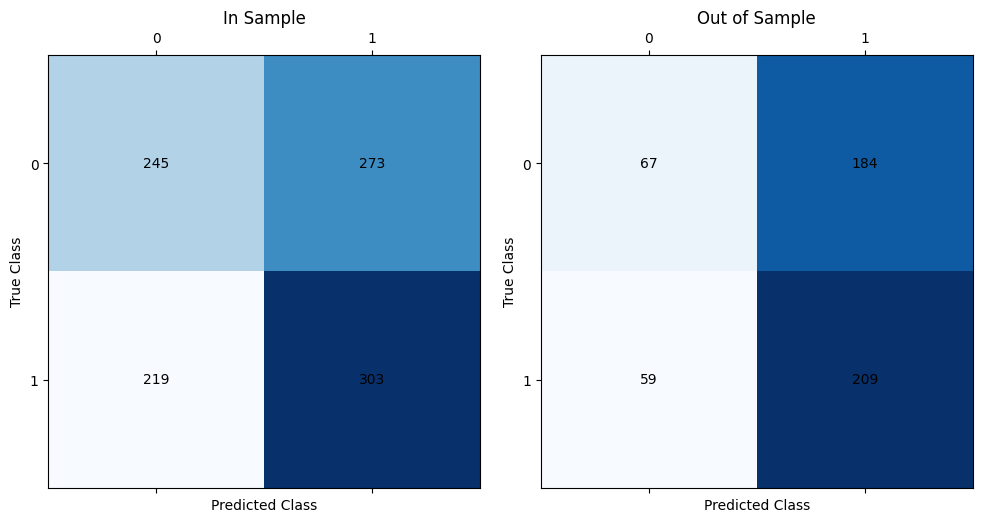
\includegraphics[width=2.60417in,height=\textheight]{graphs/scores_cm.png}

}

\caption{Scores confusion matrix}

\end{figure}

\hypertarget{interpretation}{%
\subsubsection{Interpretation}\label{interpretation}}

These results show that the model is performing at a fairly basic level,
with accuracy, precision, and recall all hovering around 53\% both
in-sample and out-of-sample. This means the model is just slightly
better than flipping a coin when it comes to predicting the correct
class. The fact that the in-sample and out-of-sample metrics are so
close is actually a good sign in terms of consistency. This suggests the
model isn't overfitting to the training data and generalizes in a
similar way to new, unseen data.

However, the relatively low F1 score, especially out of sample (about
0.498), indicates that the balance between precision and recall is not
ideal. In practical terms, this means the model is either missing some
positive cases or generating more false alarms than we'd like. While
it's encouraging that the model isn't falling apart on new data, these
metrics also tell us there's a lot of room for improvement. We might
need better features, more data, or a different model altogether to get
meaningful predictive power.

The desired results for the confusion matrix would be darker diagonals,
but since the classes are unbalanced it is harder to actually interpret
than the scores.

\hypertarget{comparing-with-the-ear}{%
\subsection{Comparing with the EAR}\label{comparing-with-the-ear}}

\hypertarget{results-1}{%
\subsubsection{Results}\label{results-1}}

We once again plot the EAR compared to time:

\begin{figure}

{\centering 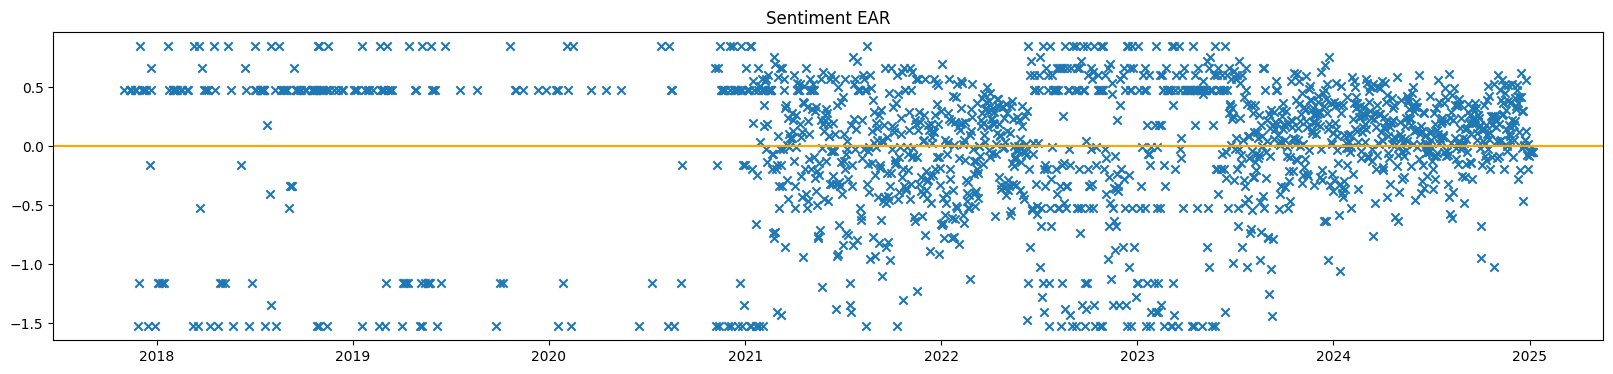
\includegraphics{graphs/ear_vs_time.png}

}

\caption{EAR vs Time}

\end{figure}

We notice the same pattern as per the score (less equally distributed
when we have less data), only a little bit reduced. This will likely
improve the results of our regression. However, we see more of a bias
towards the negative which might skew our results. This might mean that
the sentiment is more negative than expected. It is interesting to see
that the effect is not as drastic on the positive side, implying that
the AR(1) model has heteroskedasticity in the errors which are more
often negative than positive. This can reflect irrational fear or panic.
We will later be able to see in the trading strategy if we perform
better during moments of panic or during moments of overconfidence.
Given this pattern, we expect the strategy to perform better during
panics, as they are more easily picked up by the model.

We plot the distribution of the EAR:

\begin{figure}

{\centering 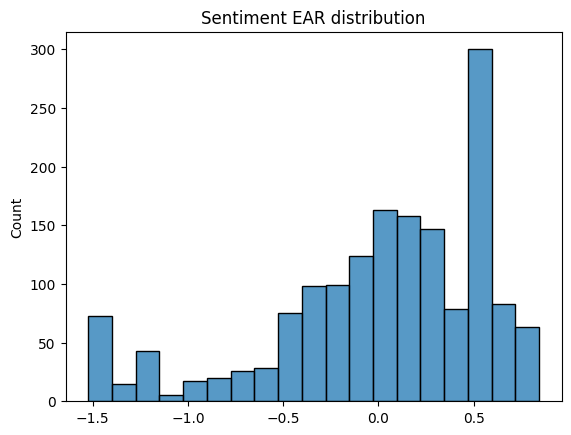
\includegraphics[width=2.60417in,height=\textheight]{graphs/ear_distrib.png}

}

\end{figure}

We see that although there are more moments when the EAR is positive,
the negative values are more drastic than the positive values. This
might indicate that the logistic regression will be only slightly better
than with the scores, given the unbalanced classes, but that the trading
strategy will perform well during panics.

We look at the scores

\begin{table}[h]
\centering
\begin{tabular}{|l|c|c|c|c|}
\hline
\textbf{Dataset} & \textbf{Accuracy} & \textbf{Precision} & \textbf{Recall} & \textbf{F1 Score} \\
\hline
In Sample & 0.5481 & 0.5494 & 0.5481 & 0.5440 \\
Out of Sample & 0.5414 & 0.5437 & 0.5414 & 0.5123 \\
\hline
\end{tabular}
\caption{Model performance metrics in and out of sample}

\end{table}

Adn the confusion matrix

\begin{figure}

{\centering 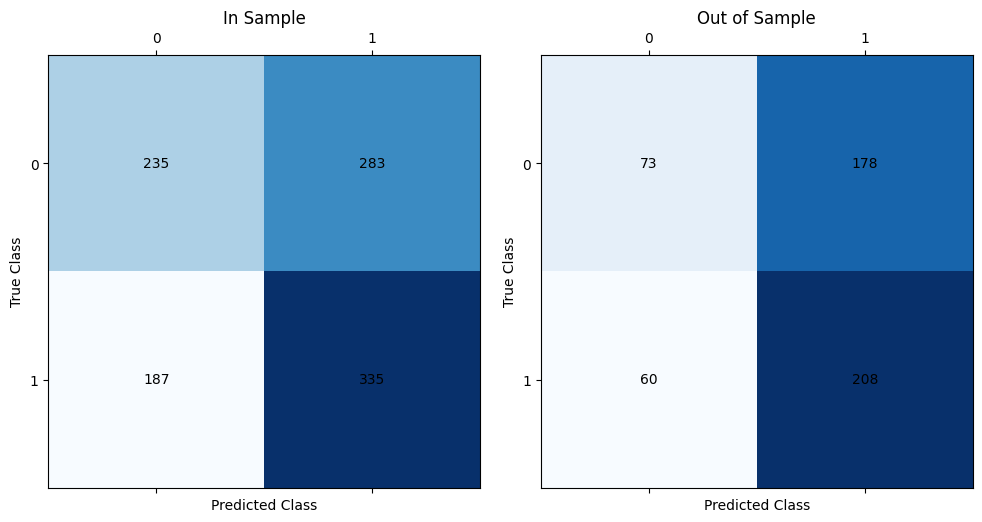
\includegraphics[width=2.60417in,height=\textheight]{graphs/ear_cm.png}

}

\end{figure}

\hypertarget{interpretation-1}{%
\subsubsection{Interpretation}\label{interpretation-1}}

We can see that the results are only slightly improved
(\textasciitilde+2\% of accuracy), but that we still have a problem with
unbalanced classes.

These updated scores show a modest improvement in the model's overall
performance. This suggests the model is doing a slightly better job of
distinguishing between the two classes and is making more reliable
predictions overall. The F1 score, which balances precision and recall,
also increased (especially in-sample) indicating that the model is
better at handling trade-offs between false positives and false
negatives.

However, while this is a step in the right direction, the gains are
still relatively small. Accuracy is still just around 54\%, which means
the model remains only marginally better than chance. The F1 score out
of sample, while improved, is still lower than the other metrics,
suggesting some imbalance or inconsistency when the model encounters new
data. So, while the improvements are meaningful and suggest progress,
there's still significant room for refinement if we want the model to be
practically useful in a high-stakes or noisy environment like financial
prediction. However, we will stick to following the methodology of the
paper for this project.

\hypertarget{trading-strategy}{%
\subsection{Trading strategy}\label{trading-strategy}}

\hypertarget{signal-with-the-irf}{%
\subsubsection{Signal with the IRF}\label{signal-with-the-irf}}

The \textbf{\emph{Impulse Response Function}}(IRF) is a way to measure
how one variable reacts over time to a sudden change in another
variable. In the context of the paper, the IRF helps us understand how
asset returns respond to unexpected changes in economic sentiment. So,
if there's a surprise jump or drop in sentiment today, the IRF tells us
what typically happens to returns in the days that follow. This is
powerful because it gives us a time-based profile of the market's
behavioral reaction to mood swings.

In trading, this is useful because if we know that sentiment shocks tend
to cause returns to go up (or down) over the next few days or weeks, we
can position accordingly: buy if returns are expected to rise, or
avoid/short if they're likely to fall. The IRF, then, becomes a kind of
``map'' for what to expect after a mood shift, and the trading signal is
built directly from that.

In the paper, the IRF is estimated using a method called local
projections. For each time horizon , \(h\) the author regresses future
returns on today's sentiment shock and current return as a control. The
general formula looks like this:

\[
\sum_{j=1}^{h} r_{t+j} = \alpha + \beta \cdot \text{EAR}_t + \gamma \cdot r_t + \varepsilon_t
\]

Here, the cumulative sum of the returns is equal to the sentiment shock
times how much the future returns move in response to that shock.

Once the IRF is estimated across multiple horizons, the paper builds a
trading signal by multiplying today's sentiment shock by the sum of
those IRF coefficients:

\[
\text{PredictedReturn}_t = \text{EAR}_t \times \sum_{h=1}^{H} \beta_h
\]

If this predicted return is positive, it suggests a favorable outlook,
and the strategy goes long. If it's negative, the model expects a drop,
and the strategy goes short or stays out. This signal is grounded in
observed market behavior rather than guesswork, which is what makes the
IRF such a compelling tool for strategy design.

\hypertarget{results-2}{%
\subsubsection{Results}\label{results-2}}

Here are the results for this strategy compared to a simple long bitcoin
portfolio :\\

\begin{figure}

{\centering 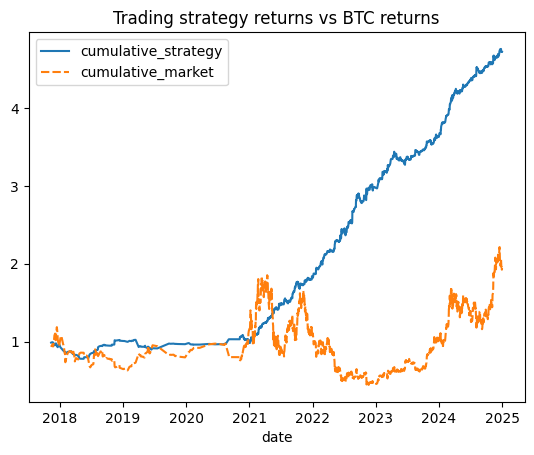
\includegraphics[width=2.60417in,height=\textheight]{graphs/strat.png}

}

\caption{Strategy vs BTC}

\end{figure}

The results here are interesting: we can see that the model only
slightly captures the rise during 2020 : this might be because of two
factors:

\begin{enumerate}
\def\labelenumi{\arabic{enumi}.}
\item
  There is less data available
\item
  BTC returns were less based on news about bitcoin itself and more on
  the current market environment (covid meant more retail investor
  participation who had a bias for bitcoin)
\end{enumerate}

Given the small variance in our strategy but undereation to 2020, we
suggest that it is a mix of both.

However, all of these results are \textbf{in-sample.}

We then look at the results with an out of sample part (30\% of the
dataset):\\

\begin{figure}

{\centering 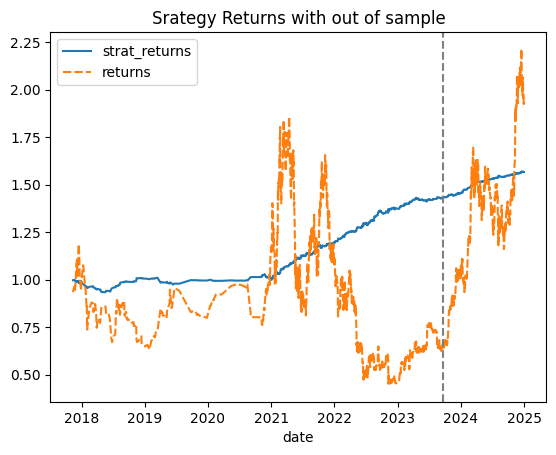
\includegraphics[width=2.60417in,height=\textheight]{graphs/strat_out_sample.png}

}

\caption{Out of sample returns}

\end{figure}

\hypertarget{interpretation-2}{%
\subsubsection{Interpretation}\label{interpretation-2}}

The first plot shows how the strategy performs across the full dataset,
including both training and test periods. It looks very strong,
consistently outperforming the market (BTC) with much less volatility.
However, since this includes the data the model was trained on, the
results may be overly optimistic and reflect some degree of overfitting
to past patterns.

The second plot gives a more realistic view by separating out the
out-of-sample period with a vertical line. Here, the strategy continues
to perform steadily but misses the sharp gains in BTC seen after 2023.
This suggests the strategy is more conservative and stable but may
underperform in strong bull markets. It's still useful for limiting
downside risk, but less effective for capturing big upside moves.
However, we saw during the trading period and during the EAR
distribution analysis that it generally performs better during panic /
crashes (where irrational sentiment might play a bigger role in returns)
than in bull markets. Therefore, we would need more data to really
conclude on the usefulness of the strategy.

It is important to note that this might however not be possible in
practice given the availability of the data in real time, the
granularity of the data, transaction costs and other factors.

\hypertarget{conclusion}{%
\section{Conclusion}\label{conclusion}}

In this project, we explored whether sentiment, specifically
expectations generated by a large language model, can help predict
Bitcoin returns and guide a trading strategy. We used the Mistral API to
extract directional views from crypto-related news headlines and turned
those into a belief-based sentiment score. From there, we built what's
called an ex-ante residual (EAR), which basically measures how
surprising or unusual the sentiment is compared to its recent trend. The
idea was that markets don't just move on news, they move on unexpected
news.

We used these EAR values to estimate how Bitcoin tends to react to
sentiment shocks over time, using impulse response functions (IRFs).
These IRFs gave us a way to forecast short-term return patterns and
build a trading signal. In backtests, the strategy performed
consistently across both in-sample and out-of-sample periods. It didn't
outperform Bitcoin during big bull runs, but it did offer more stability
and avoided sharp downturns when sentiment turned negative. That makes
it potentially useful in a volatile market like crypto.

We also tried a simple classification model to see if sentiment could
help predict crashes. The results were modest, only slightly better than
random, but they were stable across different samples, which is still a
positive sign. More importantly, both the IRF-based strategy and the
classifier showed that LLM-generated sentiment isn't just noise. It
reflects how the market feels, and when that mood shifts unexpectedly,
it often shows up in prices.

What we've built here is a simple but thoughtful approach to trading on
market psychology. There's still a lot of room for improvement, whether
that means using better data, more advanced models, or expanding to
other assets. But the foundation is solid: by listening to how people
talk about the market, we can start to get a sense of where it might go
next.

\hypertarget{bibliography}{%
\subsection{Bibliography}\label{bibliography}}


\printbibliography


\end{document}
